\section{Montering}
En hjulbas kommer att finnas tillhanda och det är på den som samtliga moduler kommer att monteras. Hjulbasen som vi kommer att använda heter Carpet Rover och är trehjulig med två drivande hjul och ett stödhjul.

\subsection{Moduler}
För att underlätta till exempel felsökning eller byte av en hel modul så kommer all hårdvara att monteras modulvis. Modulerna kommer i sin tur att monteras i tre nivåer, med undantag för sensorerna. 

\begin{figure}[H]
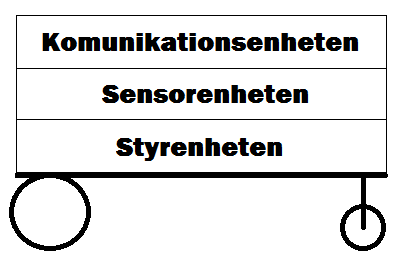
\includegraphics[angle=0,scale=0.5]{bilder/enheter.png}
  \centering
  \caption{De olika enheternas placering}
  \label{fig:enheter}
\end{figure}

\subsubsection{Styrenheten}
Underst kommer styrenheten vara monterad som består av en AVR ATmega16. Denna kommer att vara kopplad för att ta emot signaler från kommunikationsenheten och sända information till motorerna.

\begin{figure}[H]
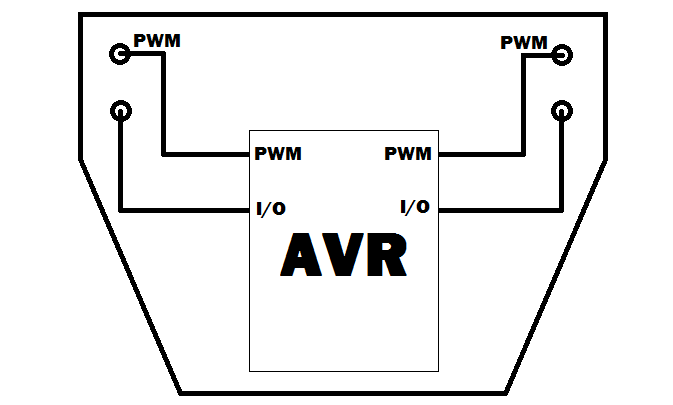
\includegraphics[angle=0,scale=0.5]{bilder/styrenhet.png}
  \centering
  \caption{Montering av styrenheten}
  \label{fig:styrenhet}
\end{figure}

\subsubsection{Sensorenheten}
På mittenplanet ska sensorenheten monteras. Den kommer att bestå av en AVR ATmega16, tre optiska avståndsmätare av typen GP2Y0A02YK (20-150 cm), en alfanumerisk LED-display av typen HDSP-2112, 11st lysdioder med 11st ljuskänsliga transistorer, en mux och en demux. AVR ATmega16 innehåller åtta portar för A/D omvandling (ADC). De optiska avståndsmätarna ska vara kopplade till ADCn. LEDn ska sedan vara kopplad till AVRn för att visa avståndsinformation. Muxen ska vara kopplad för att styra lysdioderna och ska styras av AVR:en.  De elva transistorerna ska vara kopplade till demuxen som  i sin tur är kopplad vidare till ADCn.

\begin{figure}[H]
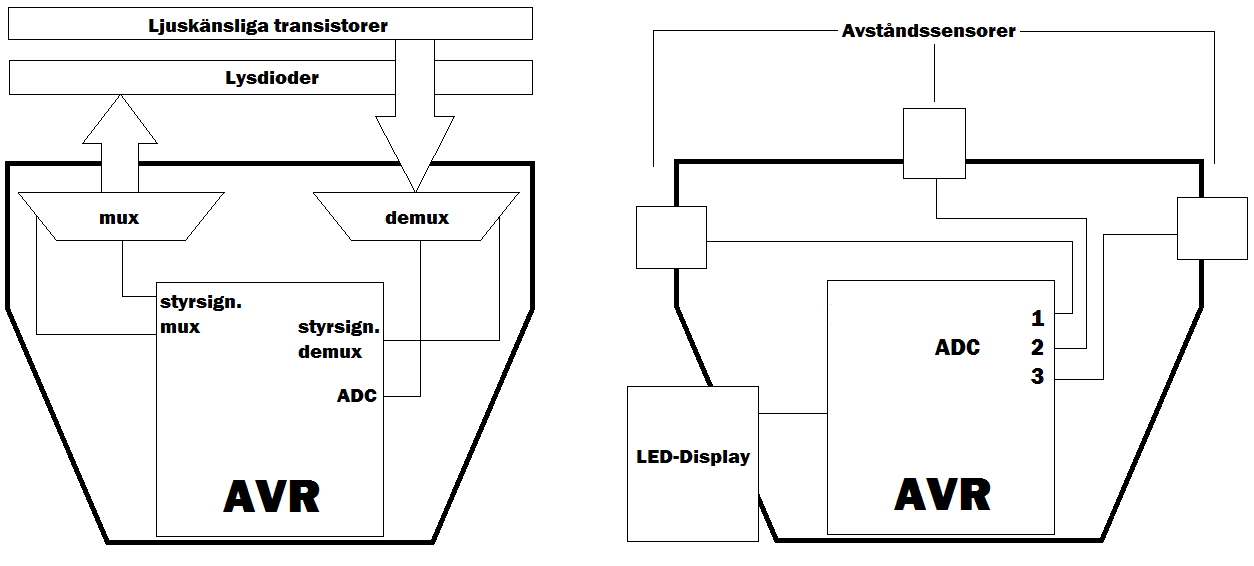
\includegraphics[angle=0,scale=0.5]{bilder/sensorer.png}
  \centering
  \caption{Montering av sensorenheten}
  \label{fig:sensorer}
\end{figure}

\subsubsection{Kommunikationsenheten}
Till kommunikationsenheten kommer en AVR ATmega16 och en FireFly enhet att användas. dessa kommer att vara monterade på översta planet på roboten. FireFlyn ska vara kopplad till AVRn via UART AVRn ska i sin tur var kopplad till de två andra enheterna.

\begin{figure}[H]
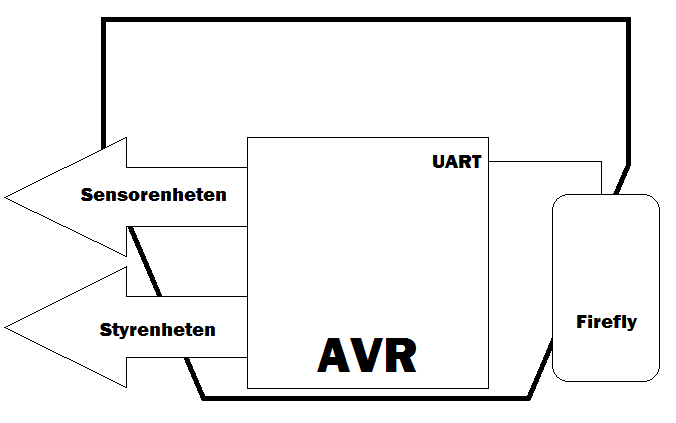
\includegraphics[angle=0,scale=0.5]{bilder/Kommunikationsenhet.png}
  \centering
  \caption{Montering av kommunikationsenheten}
  \label{fig:Kommunikationsenheten}
\end{figure}

\subsection{Sensorer}
Sensorernas montering ska förenkla för roboten ta beslut. För att maximera robotens framförhållning ska sensorerna vara monterade så långt fram som möjligt. Till exempel kan det handla om beslut för att undvika en kommande kollision.

\subsubsection{Linjesensor}
Linjesensorerna består av en 11st lysdioder med 11st ljuskänsliga transistorer. Dessa ska vara monterade parvis i en rak linje framför de två drivande hjulen på roboten. Linjesensorn ska monteras nära marken så att den ger en god signal.

\subsubsection{Avståndssensor}
De tre avståndssensorerna ska vara riktade åt var sitt håll. En ska vara riktad rakt fram, en åt höger och en åt vänster. Alla tre sensorer ska vara monterade i främre delan av roboten. Avståndsmätarna ska sedan vara kopplade till ADC på AVRn.